\documentclass[tikz,border=3pt]{standalone}
\usepackage{tikz}
\usetikzlibrary{calc}
\usetikzlibrary{angles,quotes}

\definecolor{customcolor}{rgb}{0,0.5,0}

\begin{document}
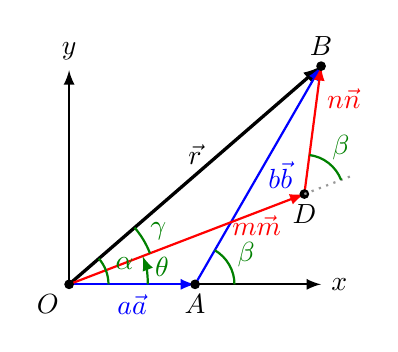
\begin{tikzpicture}[>=latex, thick, scale=1.6]

% ------------------------------------------------------------------
% === EDITABLE PARAMETERS ==========================================
\def\aInt{1}        % a  (lower‑layer coefficient of vec a)
\def\bInt{2}        % b  (lower‑layer coefficient of vec b)

\def\mInt{2}        % m  (upper‑layer coefficient of vec m)
\def\nInt{1}        % n  (upper‑layer coefficient of vec n)

\def\thetaDeg{21}   % twist angle θ in degrees  (upper layer rotation)


% \def\aInt{2}        % a  (lower‑layer coefficient of vec a)
% \def\bInt{15}        % b  (lower‑layer coefficient of vec b)

% \def\mInt{5}        % m  (upper‑layer coefficient of vec m)
% \def\nInt{13}        % n  (upper‑layer coefficient of vec n)

% \def\thetaDeg{9.43}   % twist angle θ in degrees  (upper layer rotation)
% ==================================================================
% ------------------------------------------------------------------

% --- lower‑layer primitive vectors (triangular lattice) -----------
\def\ax{1}            \def\ay{0}
\def\bx{0.5}          \pgfmathsetmacro{\by}{sqrt(3)/2}

% --- rotated upper‑layer primitive vectors ------------------------
\pgfmathsetmacro{\mx}{\ax*cos(\thetaDeg) - \ay*sin(\thetaDeg)}
\pgfmathsetmacro{\my}{\ax*sin(\thetaDeg) + \ay*cos(\thetaDeg)}

\pgfmathsetmacro{\nx}{\bx*cos(\thetaDeg) - \by*sin(\thetaDeg)}
\pgfmathsetmacro{\ny}{\bx*sin(\thetaDeg) + \by*cos(\thetaDeg)}

% --- coordinates of key points ------------------------------------
%  lower‑layer triangle O‑A‑B
\pgfmathsetmacro{\Ax}{\aInt * \ax}
\pgfmathsetmacro{\Ay}{\aInt * \ay}
\pgfmathsetmacro{\Bx}{\Ax + \bInt * \bx}
\pgfmathsetmacro{\By}{\Ay + \bInt * \by}

%  upper‑layer point D = m·m⃗
\pgfmathsetmacro{\Dx}{\mInt * \mx}
\pgfmathsetmacro{\Dy}{\mInt * \my}

% --- (optional) background grid for context -----------------------
% \draw[very thin,gray!30] (-0.5,-0.5) grid [step=0.5] (3.5,3);

% --- axes ----------------------------------------------------------
% \draw[->] (-0.5,0) -- (2.5,0) node[right] {$x$};
% \draw[->] (0,-0.5) -- (0,2) node[above] {$y$};
\draw[->] (0, 0) -- (2.0, 0) node[right] {$x$};
\draw[->] (0, 0) -- (  0, 1.7) node[above] {$y$};

% --- common radius OB ---------------------------------------------
\draw[black,very thick,->] (0,0) -- (\Bx,\By) node[midway,above] {$\vec{r}$};

% === lower‑layer triangle (blue) ==================================
%  O -> A  (a·vec a)
\draw[blue,->] (0,0) -- (\Ax,\Ay) node[midway,below] {$a\vec a$};
%  A -> B  (b·vec b)
\draw[blue,->] (\Ax,\Ay) -- (\Bx,\By) node[midway,right] {$b\vec b$};

% === upper‑layer triangle (red) ===================================
%  O -> D  (m·vec m)
\draw[red,->] (0,0) -- (\Dx,\Dy) node[pos=0.65,right] {$m\vec m$};
%  D -> B  (pretend n·vec n)
\draw[red,->] (\Dx,\Dy) -- (\Bx,\By) node[pos=0.75,right] {$n\vec n$};

% --- mark and label all vertices ----------------------------------
\fill (0,0)        circle (1.1pt) node[below left] {$O$};
\fill (\Ax,\Ay)    circle (1.1pt) node[below]      {$A$};
\fill (\Dx,\Dy)    circle (1.1pt) node[below]      {$D$};
\fill (\Bx,\By)    circle (1.1pt) node[above]      {$B$};

\coordinate (O) at (0,0);
\coordinate (A) at (\Ax,\Ay);
\coordinate (B) at (\Bx,\By);
\coordinate (D) at (\Dx,\Dy);
\coordinate (x) at (2,0);
\coordinate (H) at ($1.2*(D)$);



\draw[dotted, black!40] (D) -- ($1.2*(D)$);


\draw pic[
    draw=customcolor,
    -,
    angle eccentricity=1.5,
    angle radius=0.5cm,
    "$\textcolor{customcolor}{\beta}$"
] {angle = x--A--B};


\draw pic[
    draw=customcolor,
    -,
    angle eccentricity=1.5,
    angle radius=0.5cm,
    "$\textcolor{customcolor}{\beta}$"
] {angle = H--D--B};


\draw pic[
    draw=customcolor,
    -,
    angle eccentricity=1.5,
    angle radius=0.5cm,
    "$\textcolor{customcolor}{\alpha}$"
] {angle = x--O--B};


\draw pic[
    draw=customcolor,
    -,
    angle eccentricity=1.2,
    angle radius=1.1cm,
    "$\textcolor{customcolor}{\gamma}$"
] {angle = D--O--B};


\draw pic[
    draw=customcolor,
    ->,
    angle eccentricity=1.2,
    angle radius=1cm,
    "$\textcolor{customcolor}{\theta}$"
] {angle = A--O--D};




\end{tikzpicture}
\end{document}
